\section{System Architectures}\label{sec:systems}

\textbf{Generate broadly, filter hard.} The industrial systems we found share one shape, shown in Fig.~\ref{fig:pipeline}: a context builder feeds a generator, and one or more explicit precision gates follow before comments reach developers. Examples are BitsAI-CR's ReviewFilter \cite{sun2025bitsai}, RovoDev's LLM judge plus a learned gate \cite{tantithamthavorn2026rovodev}, AutoCommenter's confidence thresholds \cite{vijayvergiya2024aiassisted}, and the Meta-Reviewer and Validator stages of the ICML 2025 pipeline \cite{lu2025towards}. Free-form multi-agent conversation appeared in no industrial report.

\begin{figure}[t]
\centering
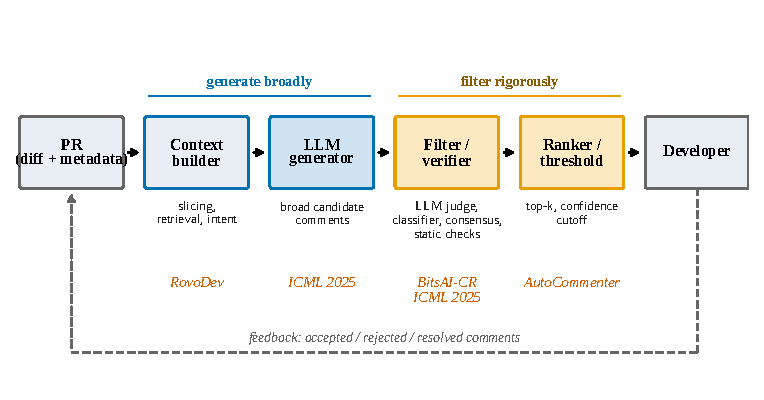
\includegraphics[width=\linewidth]{figures/pipeline.pdf}
\caption{The ``generate broadly, filter hard'' pipeline, with example systems under each stage.}
\label{fig:pipeline}
\end{figure}

\textbf{Architecture families.} The literature contains nine recurring designs, including fine-tuned detector plus verifier, multi-role pipelines with slicing and validation, a single context-aware call with judge and gate, bounded-tool agents, LLM plus static analysis, mixture of prompts, threshold-based prediction and multi-run aggregation.

\textbf{Purpose-built versus general agents.} On AACR-Bench, Claude Code produced only about 0.09--0.15 comments per patch, with high precision and low recall \cite{zhang2026aacrbench}. OpenCodeReview, an unrefereed preprint, reports SEM-F1 of 25.10\% against 11.57\% for the same Claude-4.6-Opus model inside Claude Code, using 5--15$\times$ fewer tokens \cite{li2026opencodereview}. The authors are largely Alibaba-affiliated and evaluate on an Alibaba-built benchmark.

\textbf{Selective versus exhaustive context.} More context is not automatically better. On AACR-Bench, adding top-3 BM25 contexts dropped Claude's F1 from 14.46 to 9.98 \cite{zhang2026aacrbench}. On SWE-PRBench, a 2,000-token diff-plus-summary prompt beat a 2,500-token full-context prompt for every model \cite{kumar2026swe}. What is chosen seems to matter more than how much, but no controlled, cost-reporting ablation exists.

\textbf{Verifiers always cost recall.} BitsAI-CR's ReviewFilter moved offline precision/recall from 57.03/45.50 to 65.59/39.77 \cite{sun2025bitsai}, and the ICML authors note that self-correction can discard critical bug-detecting comments \cite{lu2025towards}. Independence helps: Claude reviewing Codex drafts raised the pass rate from 71.6\% to 89.7\%, Codex reviewing Claude drafts lowered it from 91.4\% to 82.8\%, and Claude's self-review changed nothing \cite{xiang2026crossmodel}. Consensus is not truth: ten dedicated reviewers unanimously endorsed a non-existent OpenSSL padding oracle, and only an empirical test killed it \cite{agarwal2026refute}.

\textbf{Static-analysis triage.} When the LLM adjudicates one bounded question about a single warning, results are strong. At Tencent, hybrid LLM and static-analysis techniques removed 94--98\% of false positives while maintaining high recall, at \$0.0011--\$0.12 per alarm \cite{du2026reducing}. The lesson is to give the LLM narrowly scoped adjudication tasks and leave candidate generation to deterministic analysers where possible.
